\section{Method}\label{sec:method}

Our system comprises a variety of off-the-shelf components:

\begin{itemize}
\item Microsoft Active Directory with LDAP support
\item Raspberry Pi connected to an RFID door entry system (see
  Fig.~\ref{fig:raspberry-pi-rfid})
\item Progress Kemp LoadMaster~\cite{progress-kemp-loadmaster-xx}
\item Progress WhatsUp Gold~\cite{progress-kemp-whatsup-gold-xx}
\item Web servers (Apache HTTP Server)
\end{itemize}

\subsection{Microsoft Active Directory With LDAP Support}

\begin{figure}
  \centerline{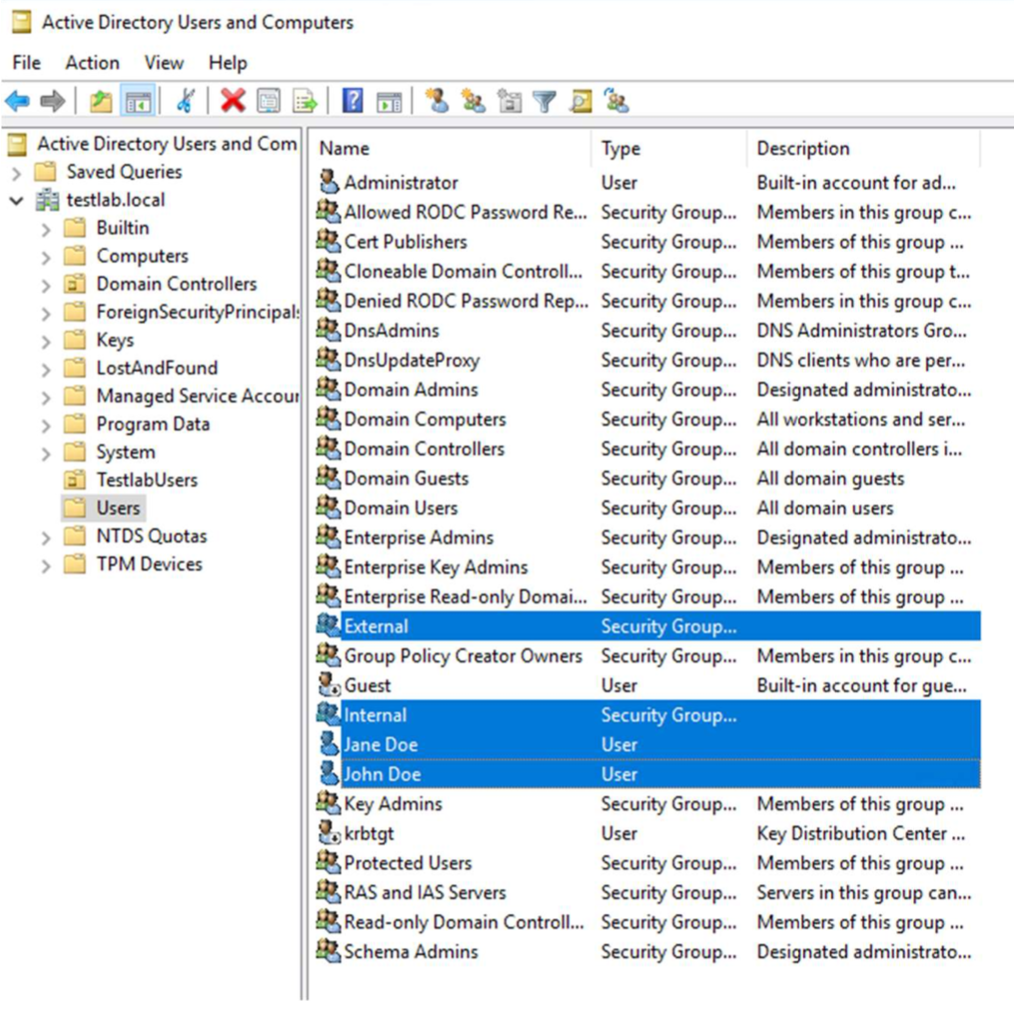
\includegraphics[width=\columnwidth]{img/active-directory}}
  \caption{We created two users, Jane Doe and John Doe, and two
    groups, Internal and External, in Active
    Directory.}\label{fig:active-directory}
\end{figure}

We used Microsoft Windows Server 2019 to run a Domain Controller (DC)
(\texttt{d1.testlab.local}) for our domain (\texttt{testlab.local}).
This is the primary DC for the scenario and it was setup to host
Active Directory (AD) with LDAP support and the Domain Name System
(DNS).  To ensure that the requests for the Web resources went to the
appropriate services on the Progress Kemp LoadMaster, we created
corresponding DNS delegations.  This is important as we wanted the
external requests to be pointed to the external resources and the
internal requests to be pointed to the internal resources.  It also
allows the LoadMaster to perform service health checks before
responding to DNS requests thus preventing IP addresses being returned
when resources are unavailable.  We added two users, Jane Doe and John
Doe, and two groups, Internal and External, to AD (see
Fig.~\ref{fig:active-directory}).

\subsection{Raspberry Pi and RFID Door Entry System}

\begin{figure}
  \centerline{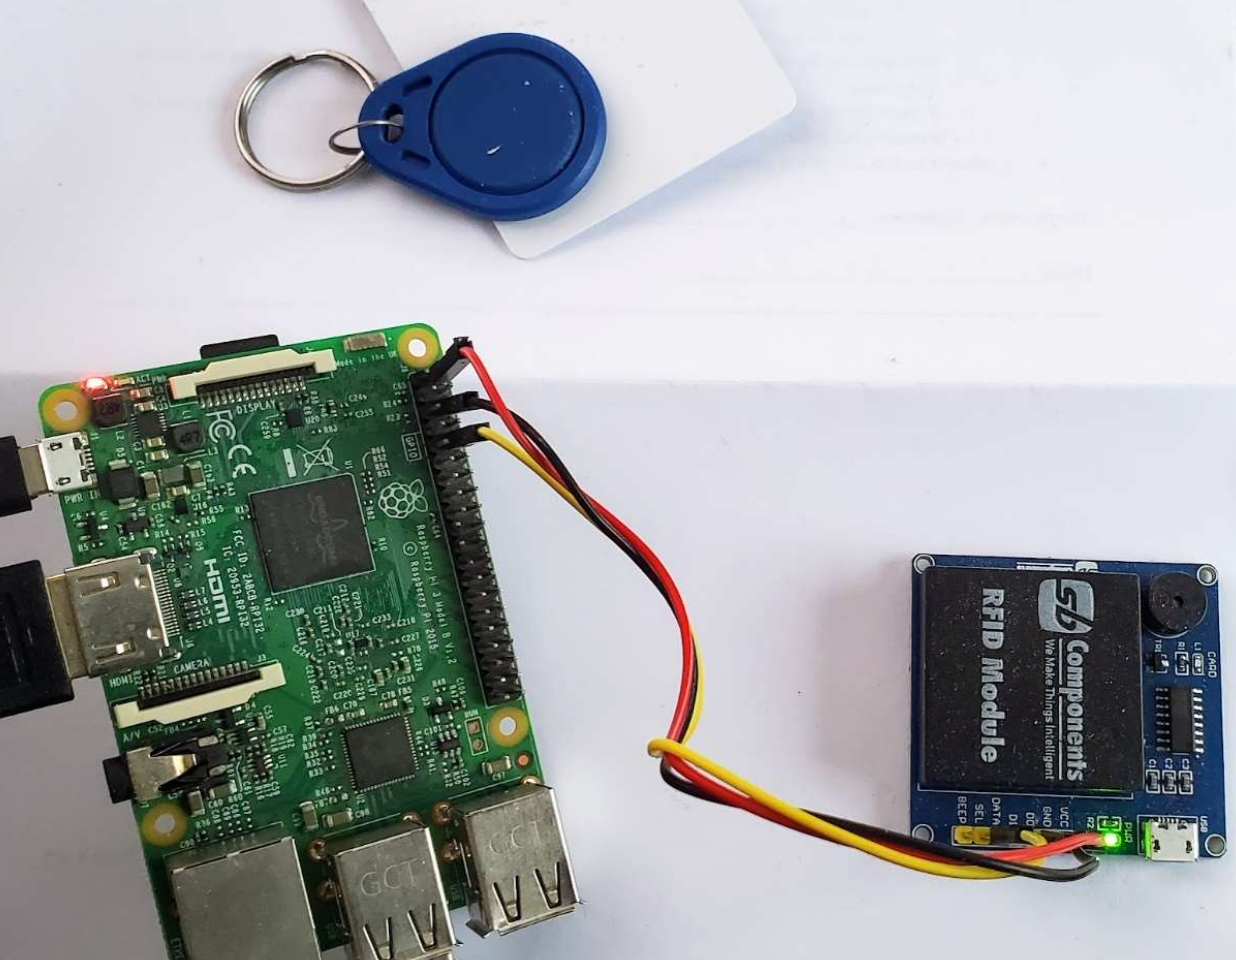
\includegraphics[width=\columnwidth]{img/raspberry-pi-rfid}}
  \caption{The Raspberry Pi was connected to an RFID door entry
    system.  We created a Python script that read the identification
    details from swiped cards and interacted with Active
    Directory.}\label{fig:raspberry-pi-rfid}
\end{figure}

The Raspberry Pi is connected to an RFID door entry system.  When a
user performs a card swipe, a Python script running on the Raspberry
Pi reads the identification details from the card and remotely changes
the group membership of the user in AD.  If the user is entering the
building their group membership is changed from External to Internal;
if they are leaving the building it is changed from Internal to
External.  It logs the event to a SIEM service (see
Sect.~\ref{sec:wug}).

\subsection{Progress Kemp LoadMaster}

Progress Kemp LoadMaster (LM) is a reverse proxy and load balancer.
It has many capabilities but for this scenario we are interested in
the Edge Security Pack (ESP), the source IP blacklist from the GEO
component, and the Web Application Firewall (WAF).  We use the ESP for
Single Sign-On (SSO) for HTTP(S) services and to communicate with the
AD for both for logon and group memberships.  This pre-authenticates a
user before they gain access to a resource.  We also enabled
\textit{group steering} on the ESP: this allows LM to send traffic to
particular services based on their group membership in AD and goes
beyond the normal use of groups to simply allow or deny access.

\begin{figure*}
  \centerline{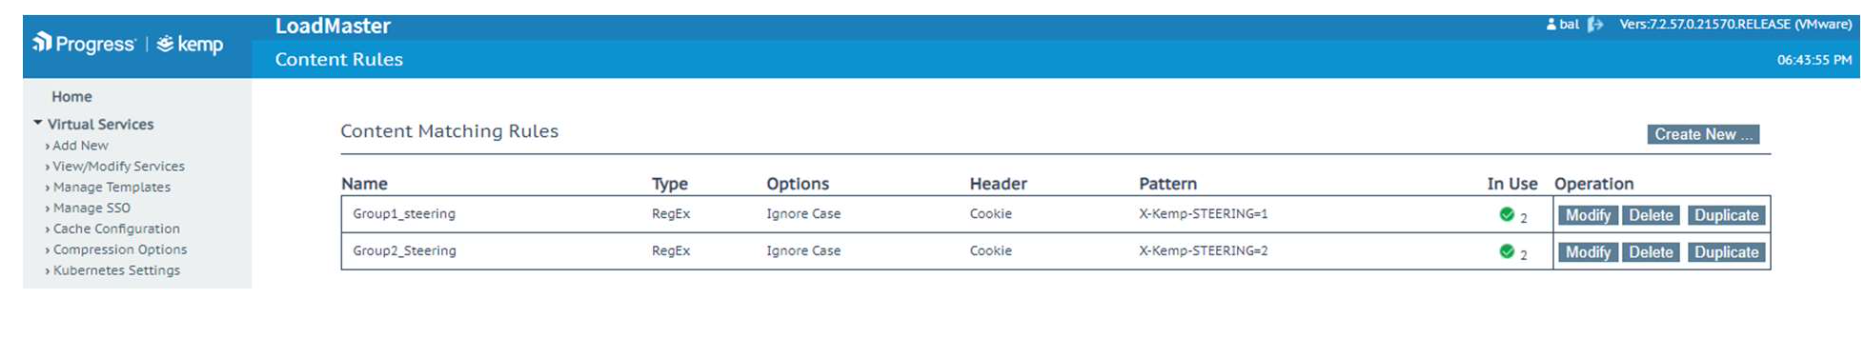
\includegraphics[width=\textwidth]{img/loadmaster-pcre-rules}}
  \caption{...}\label{fig:loadmaster-pcre-rules}
\end{figure*}

We created two steering groups associated with the Internal and
External groups in AD.  We created Perl Compatible Regular Expression
(PCRE) rules to match the authorisation cookies and steer the requests
to the appropriate services (see
Fig.~\ref{fig:loadmaster-pcre-rules}).

The login page that is displayed by the ESP is the same for both
\textit{valid} and \textit{invalid} access attempts.  A valid access
attempt occurs when a user's group and request are both internal or
both external; otherwise the access attempt is invalid.  In both cases
a log is sent to a SIEM service (see Sect.~\ref{sec:wug}).  This helps
with threat hunting as a threat actor will get the same login page for
the honey pot as with the valid site.  The honey pot can gather the
details of the access attempt without being discovered.

\begin{figure*}
  \centerline{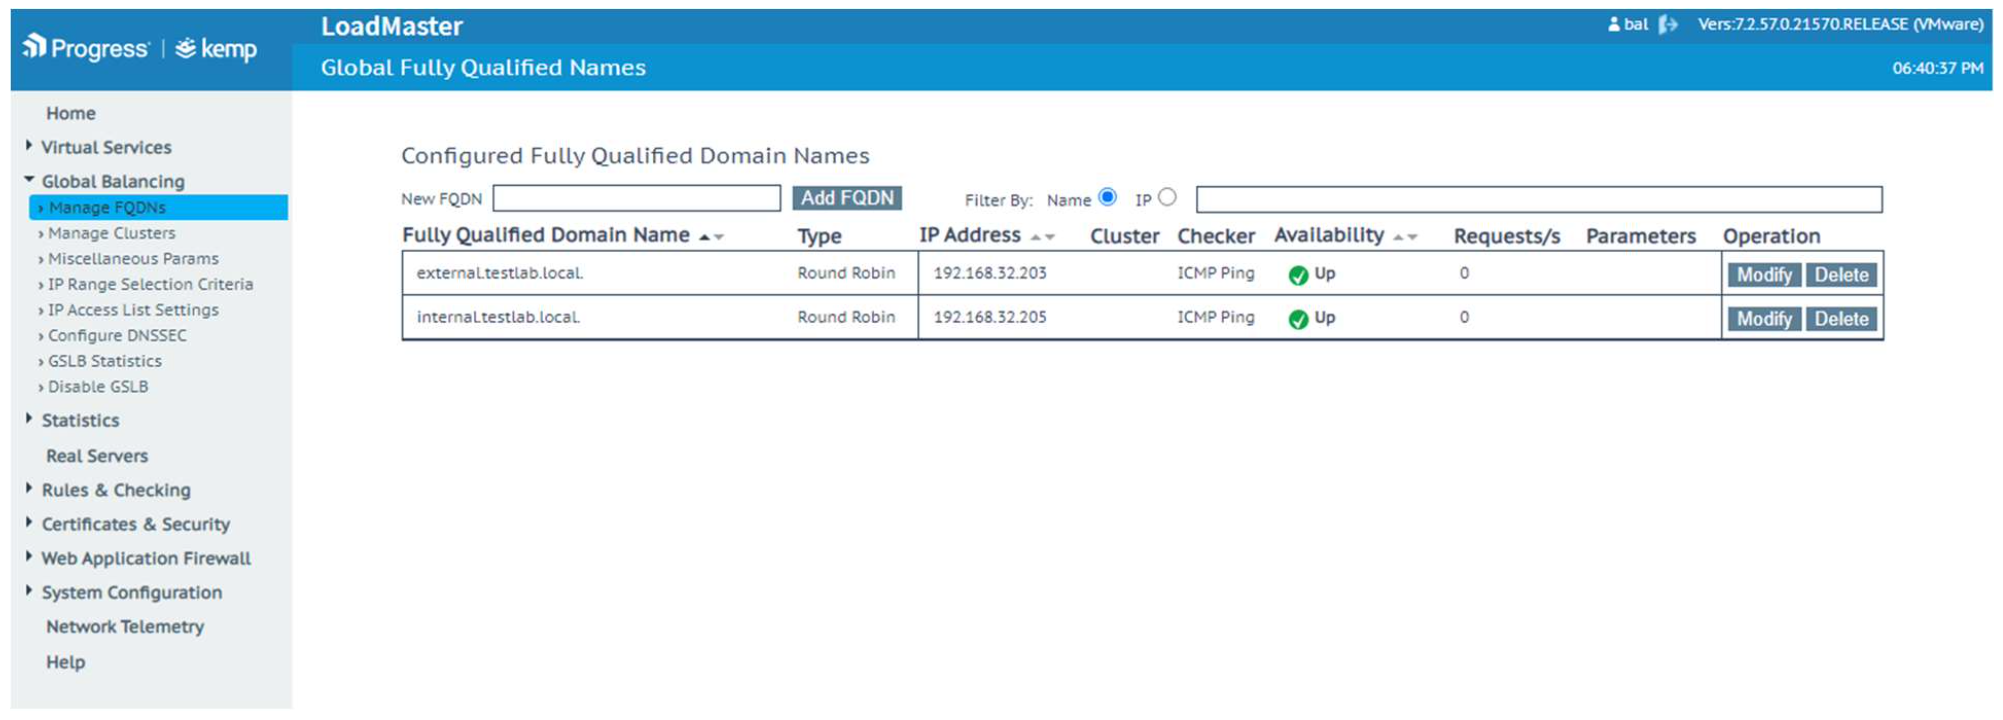
\includegraphics[width=\textwidth]{img/loadmaster-geo}}
  \caption{We configured two FQDNs for \texttt{internal.testlab.local}
    and \texttt{external.testlab.local} using LoadMaster's GEO
    component.}\label{fig:loadmaster-geo}
\end{figure*}

The GEO component performs DNS resolution and service health checks
before returning a result.  We created GEO DNS entries for
\texttt{internal.testlab.local} and \texttt{external.testlab.local}
(see Fig.~\ref{fig:loadmaster-geo}).  We also used an IP blacklist
that is updated daily to withhold DNS results from anyone on the list.

\begin{figure*}
  \centerline{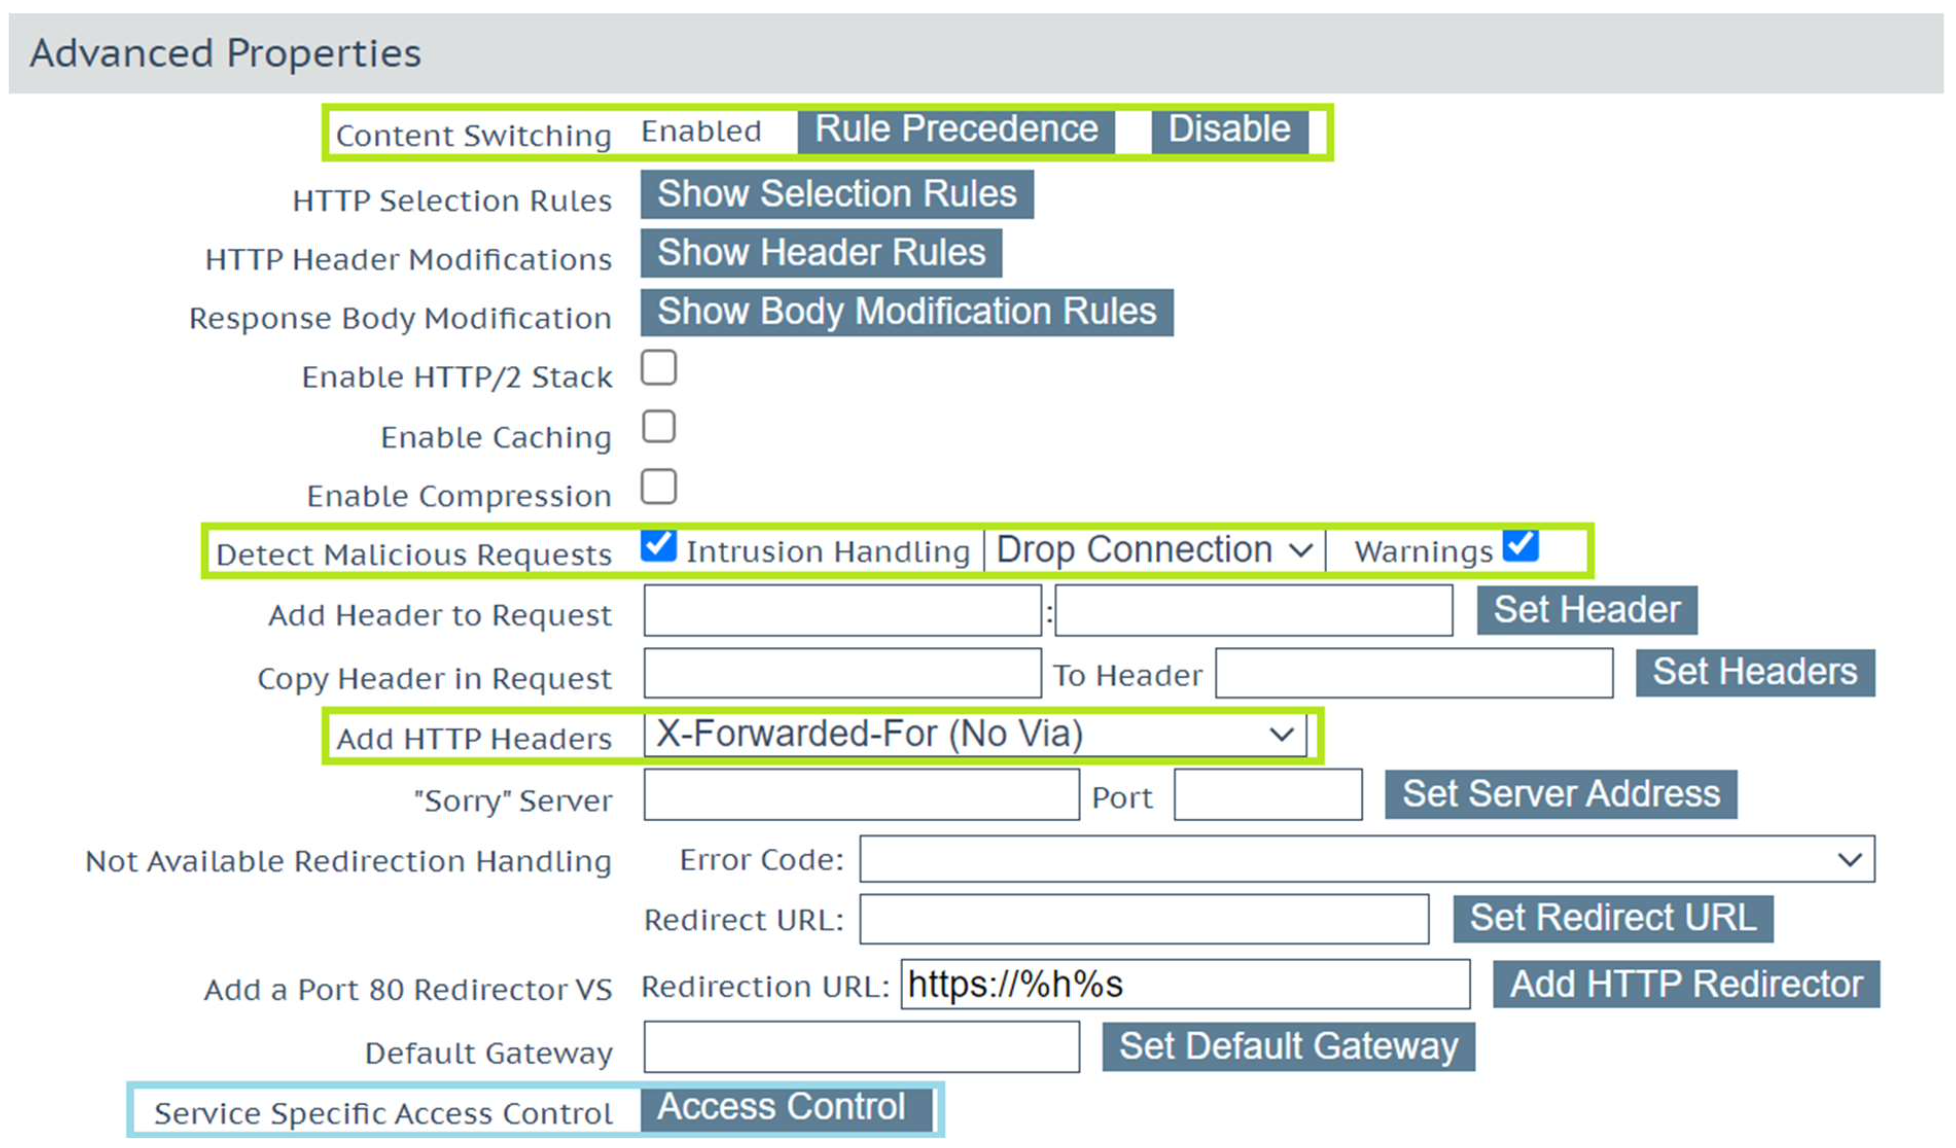
\includegraphics[width=\textwidth]{img/loadmaster-ids-ips}}
  \caption{We enabled IDS/IPS in LoadMaster as an additional layer of
    defence for little configuration.}\label{fig:loadmaster-ids-ips}
\end{figure*}

Additionally, we enabled the Intrusion Detection System (IDS) and
Intrusion Prevention Systems (IPS) on LM.  This includes rules defined
by the SNORT community~\cite{cisco-snort-xx} and enables the SNORT
rule filtering on the Layer 7 HTTP engine to check for any known bad
requests.  Figure~\ref{fig:loadmaster-ids-ips} shows the configuration
highlighted in green.  There is also an option to prevent access via
whitelists and blacklists highlighted in blue.

Finally, we enabled the Web Application Firewall (WAF) and the Open
Web Application Security Project (OWASP) core rule set.  This rule set
performs anomaly scoring and identifies, for each request, the
probability that it is malicious.  The core rule set protects against
SQL injection, cross-site scripting, remote code execution, buffer
overflows, known vulnerabilities, and many other vectors of attack.
We configured the WAF with source IP reputation blocking enabled which
uses a global IP reputation list that is updated daily. Using the
MaxMind~\cite{maxmind-xx} and the GEO component, it identifies the
country of the source request and it can be configured to block
specific countries or regions.

\subsection{Web Servers}

Our Web servers are hosted on virtual running Debian and a default
installation of the Apache HTTP Server.  The landing page is our
``valid access'' page and represents our secured Web resource.  The
``invalid access'' page is served by a Flask application.  It records
the username and source IP of all requests and sends those details to
a SIEM service (see next section).

\subsection{Progress WhatsUp Gold}\label{sec:wug}

\begin{figure*}
  \centerline{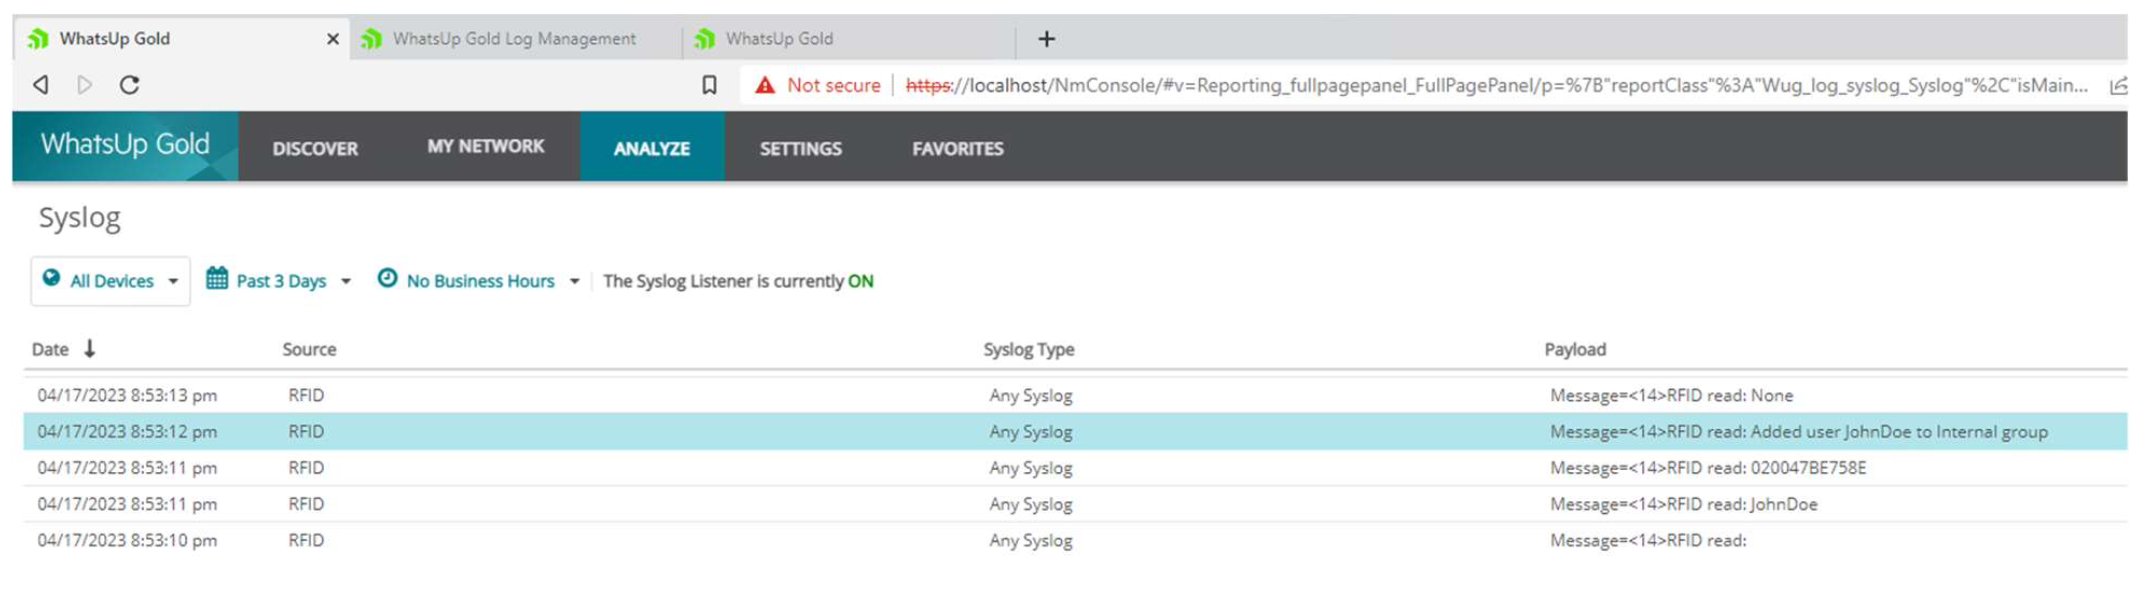
\includegraphics[width=\textwidth]{img/whatsup-gold}}
  \caption{...}\label{fig:whatsup-gold}
\end{figure*}

The Raspberry Pi, LM, and Flask application send logs to a SIEM
service.  We use Progress WhatsUp Gold (WUG) (see
Fig.~\ref{fig:whatsup-gold}).  In normal operation the events from the
Raspberry Pi, RFID door entry system, and LM are logged.  In cases
where a user's credentials may be compromised, the Flask application
logs an event with high priority.
